\chapter{Background}
\label{Chapter2}

%%%  ===========================================================================
%%%  ===OVERVIEW================================================================
%%%  ===========================================================================
\section{Overview}
This section explains the main concepts and tools needed to conduct the $\plonk$ protocol. As already mentioned $\plonk$ will have trusted setup which is one-time and updatable. Obviously, the natural benefit is that the setup parameters could be used indefinitely but furthermore this also enables $\plonk$ to be a multi-party protocol. This is the key property that makes the protocol useful and promising for application in block-chain technologies. It is important to mention that the security is based on hardness of a problem that is not post-quantum meaning that it is not safe against attack of quantum computers. $\plonk$ already has other variations like HyperPlonk \cite{HyperPlonk}, plookup \cite{plookup} which mainly introduce optimizations to the protocol. The original paper uses KZG \cite{KZG} (Kate, Zaverucha, Goldberg) commitments but the protocol could be altered to use, FRI. 

The complexity of the protocol is most usually based on a security parameter $\lambda$, which says that the size of field is at least $2^{\lambda}$. This will be clarified later for now take it as size of a domain. For example when picking a password the security parameter could be the minimal length of a password. The longer the password is the harder it is for an adversary to guess it. To give you a basic idea on complexity of $\plonk$ and how compares to other zero-knowledge protocols, take a look at the following table.

\hl{this information was stolen from zk-whiteboard presentation}
\begin{table}[h]
    \centering
    \resizebox{\textwidth}{!}{
        \begin{tabular}{ c | c c c c}
            protocol & proof size & public parameters & verifier time & trusted setup \\ 
            \hline
            Groth16      & $O_{\lambda}(1) \approx 200$ B            & $O_{\lambda}(|C|)$ & $O_{\lambda}(1) \approx 3ms$           & per circuit \\ 
            Plonk & $O_{\lambda}(1) \approx 400$ B            & $O_{\lambda}(|C|)$ & $O_{\lambda}(1) \approx 6ms$           & universal \\ 
            Bulletproofs & $O_{\lambda}(\log{|C|}) \approx 1.5$ kB   & $O_{\lambda}(1)$   & $O_{\lambda}(|C|) \approx 1.5s$        & no\\ 
            STARK        & $O_{\lambda}(\log^2{|C|}) \approx 80$ kB  & $O_{\lambda}(1)$   & $O_{\lambda}(\log{|C|}) \approx 10ms$  & no \\ 
            DARK         & $O_{\lambda}(\log{|C|}) \approx 10$ kB    & $O_{\lambda}(1)$   & $O_{\lambda}(\log{|C|})$               & no \\ 
        \end{tabular}
    }
    \caption{Comparison of protocols}
\end{table}

First let's start with a very rough idea of what.Say there exists a problem that the prover can solve and he has a solution. However, he does not want to share the solution, but just convince others that he has the solution. Cryptographers would say, he wants to provide an argument of knowledge.

What can the prover do about it? First, let's say that the prover has a solution to a problem named $P$ and there exists a computer program $Check_P$ that checks if a solution given at the input is valid. Let's say that $Check_P$ outputs 0 if and only if the input is valid solution of $P$. Now we can rephrase the task. \textbf{The prover would like to convince others that running his solution of $P$ on $Check_P$ outputs 0}. And if the program outputs 0 then the solution should be valid. This of course goes under the assumption that the others trust $Check_P$ and know that it correctly checks inputs for the problem $P$. In practice, this program is usually public meaning others can freely look at it and inspect it if wanted. 

\begin{figure}[H]
    \centering
    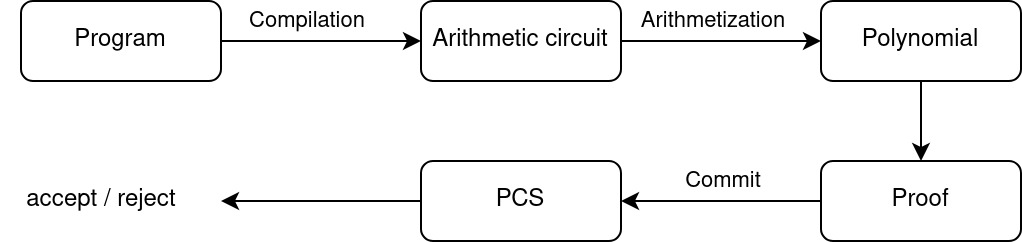
\includegraphics[width=0.75\linewidth]{figures/diagram_owerview.jpg}
    \caption{Enter Caption}
    \label{fig:entabel}
\end{figure}

At this point, the protocol might still feel a bit abstract. We can illustrate it in the famous \href{https://en.wikipedia.org/wiki/Sudoku}{Sudoku game}. In this context, the program will check if the filled table is a valid Sudoku solution by verifying that no number repeats in any row or column. The public input is the dimension of the table and a couple of the pre-filled numbers. The solution (the private information) is the remaining numbers that need to be filled. The prover claims that he knows a valid solution so he takes the program that checks the solution and rewrites it in terms of polynomials and somehow generates proof that the program would accept his solution. The proof is sent to the verifier who decides if the proof is valid. Remember that this proof is weirdly encoded and mangled in polynomials and it makes sure that the verifier does not get to know anything about the actual solution. 

At this point, the protocol might still feel a bit abstract. We can illustrate it in the famous Sudoku game. In this context, the program will check if the filled table is a valid Sudoku solution by verifying that no number repeats in any row or column. The public input is the dimension of the table and a couple of the pre-filled numbers. The solution (the private information) is the remaining numbers that need to be filled. The prover claims that he knows a valid solution so he takes the program that checks the solution and rewrites it in terms of polynomials and somehow generates proof that the program would accept his solution. The proof is sent to the verifier who decides if the proof is valid. Remember that this proof is weirdly encoded and mangled in polynomials and it makes sure that the verifier does not get to know anything about the actual solution. 

\begin{figure}[H]
    \centering
    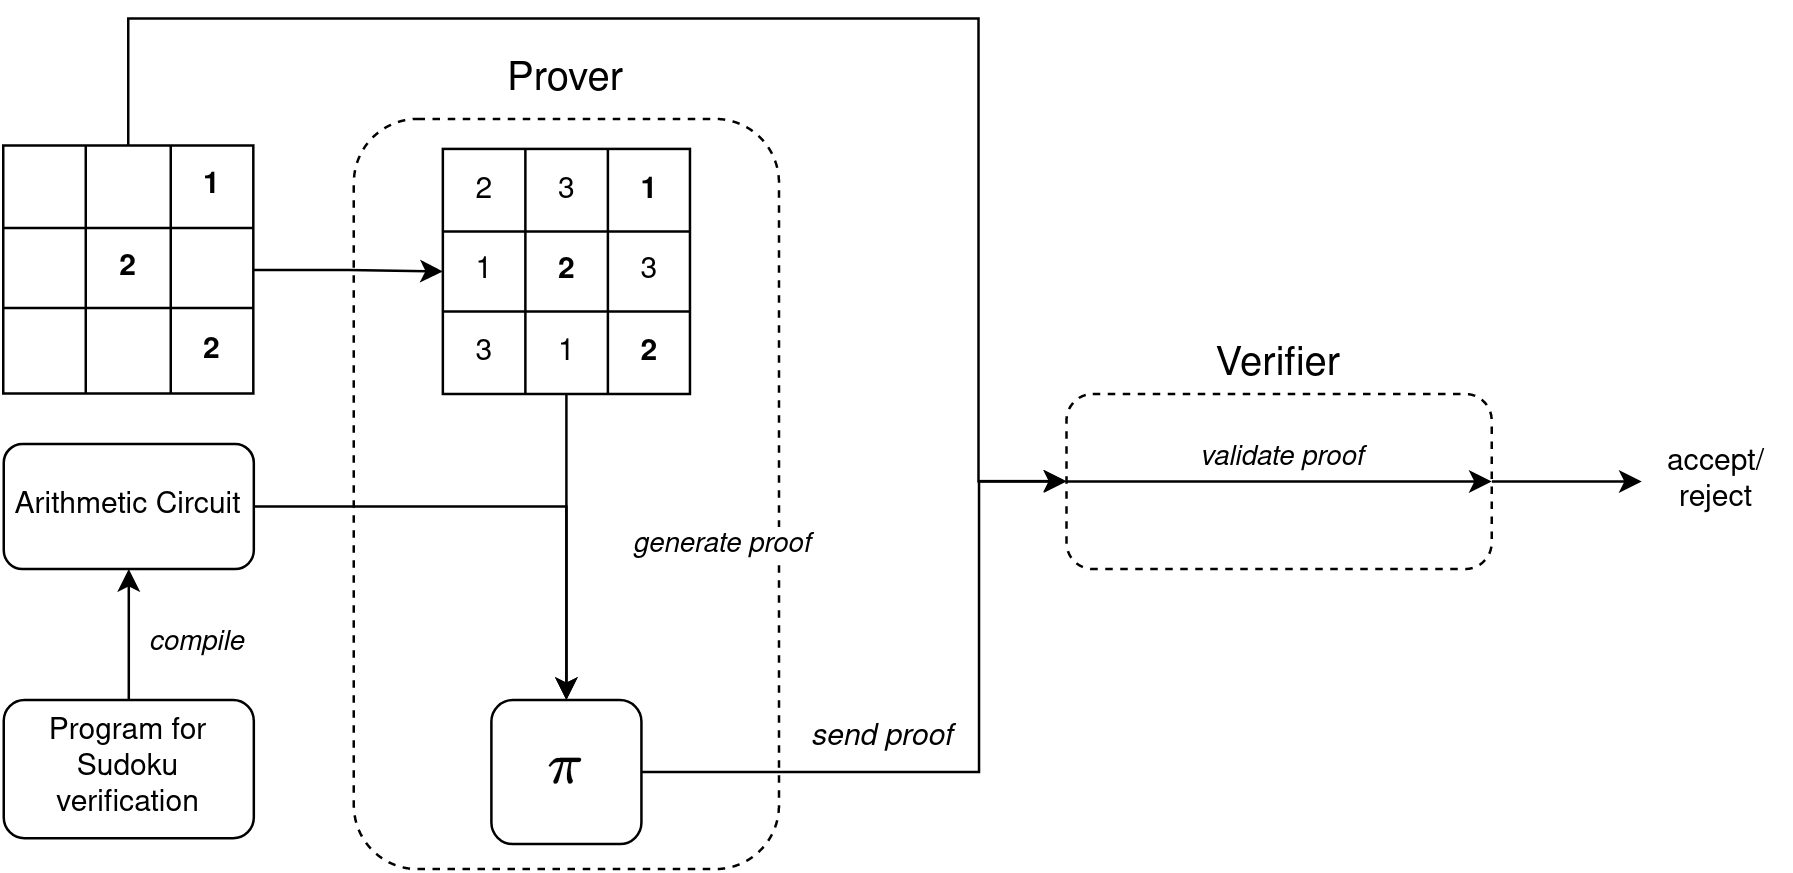
\includegraphics[width=0.75\linewidth]{figures/sudoku.drawio.png}
    \caption{Sudoku Example}
\end{figure}

\begin{enumerate}
    \item Encode circuit with secret and public parameters into polynomials
    \item Generate a proof that this encoding was indeed done correctly
    \item Verify that the proofs are valid
\end{enumerate}



% %%%  ===========================================================================
% %%%  ===POLYNOMIALS=============================================================
% \section{Polynomials}
% % % \hl{reference how snarks work}
% Polynomials are mathematical objects studied for centuries, throughout this time we have figured out many nice and even some useful properties about them. One might ask what is so special about polynomials and it turns out a lot. They serve as a good tool for representing end encapsulating circuits. Let's show a simple observation:

% \begin{lemma}{Intersection of polynomials} \newline
%     Arbitrary two polynomials in form $a_0 + a_1x + a_2x^2 ... a_nx^n = 0; b_0 + b_1x + b_2x^2 ... b_m x^m = 0$ where both $n, m \leq d \in \mathbb{N}$ intersect in no more than $d$ points.
% \end{lemma}

% \begin{dukaz} \newline
%     To find the intersection points we need to solve equation $a_0 + a_1x + a_2x^2 ... a_nx^n = b_0 + b_1x + b_2x^2 ... b_m x^m$ which will produce yet another polynomial of degree $max(n,m) \leq d$. From the Fundamental Theorem of Algebra we know that a polynomial of degree $d$ cannot have more than $d$ roots.
% \end{dukaz}

% This a simple yet incredibly crucial observation for most of the proofs that will be carried out in this article. You can think about it as a tool for probabilistic polynomial identity testing, thanks to which we can effectively compare of two polynomials just by evaluating them at a uniformly random point. If polynomials are different we know they could intersect in at most $d$ points. The probability of randomly picking one of these points is $d$ divided by size of the domain. Depending on reasonably chosen parameters usually give negligible chances to guess the point correctly. Keep in mind the the domain size is given by $\lambda$. The observation can be generalized on multi-variate polynomials by Schwartz-Zippel lemma. % % \hl{include citation} To better understand how it works we will look at series of toy protocols, where we improve their faults in iterative manner. We will start with the most simple and crappy one:

% \begin{example} \textit{Polynomial Identity Check}

%     There is a verifier who knows some polynomial $p(x)$ and prover who wants to claim that he also knows coefficients of the polynomial $p(x)$. Say the polynomial has degree $d$ and the domain or evaluation range is $[1, 2^n]$. The prover could convince verifier as follows:
    
%     \begin{enumerate}
%         \item $V$ samples random point $r \in [1, 2^n]$
%         \item $V$ sends the point $r$ to $P$
%         \item $P$ sends back evaluation $p(r)$
%         \item $V$ locally computes $p(r)$ compares to what he got from $P$
%     \end{enumerate}    
% \end{example}

% With each $i$ iterations of this protocol the prover has probability of $(\frac{d}{2^{\lambda}})^i$ of guessing correctly. While this protocol is an interesting proof of concept, by itself it does not achieve much. Both of the parties know the same polynomial the only advantage is that the verifier does not compare coefficients of the polynomial but just one point. What might sound a bit more interesting is that a prover might be able to show that his polynomial $p(x)$ can be factored by $t(x)$ into $p(x) = t(x)h(x)$. 

% \begin{example} \textit{Polynomial Factor Check}

%     P wants to convince $V$ that he knows a polynomial $p(x)$ of degree $d$ with factor $t(x)$. In this protocol $P$ does not want to share $p(x)$ but wants to prove $p(x) = t(x)h(x)$, so naturally $V$ knows $t(x)$.
%     \begin{enumerate}
%         \item $V$ samples a random point $r$
%         \item $V$ sends the point $r$ to $P$
%         \item $P$ performs polynomial division $h(x) = \frac{p(x)}{t(x)}$ and sends evaluations of $p(r), h(r)$ to back to $V$
%         \item $V$ locally evaluates $t(r)$ and checks if $p(r) = t(r)h(r)$
%     \end{enumerate}
% \end{example}

% The protocol relies on the fact that $P$ is able to divide $p(x)$ if and only if $t(x)$ indeed is co-factor. Now we have a protocol in which the verifier is not revealed polynomial $p(x)$ and can relatively succinctly verify if it has some factor so all look good. Or does it? Well, no this protocol is terrible. The verifier gets to know some information about $p$ and that is the evaluation at $r$ and what is much worse the $P$ can cheat very easily in number of different ways:

% \begin{enumerate}
%     \item $P$ does not need to know the coefficients of $p$. He can quite easily calculate evaluation $t = t(r)$ and choose $h(r)$ such that $p(r) = t(r)h(r)$, without the verifier knowing.
%     \item $P$ nothing stops the prover from changing the $p$ on the fly. He know $r$ therefore, it is easy to construct any polynomial which has one shared polynomial with $t(r)h(r)$.
%     \item Nothing is constraining the $P$ to use polynomial of degree $d$. Prover can cheat by using polynomial $\Tilde{p}(x) = p(x)h'(x)$ with arbitrary $h'(x)$ that has bigger degree and also satisfies the factor check.
% \end{enumerate}

% The first two exploits possible because the prover knows $r$ and $t(r)$, thus he can temper with the protocol. Instead we would like to provide encrypted $r$ to the prover, so that he can use it as black box but does not know the real value. We will tackle this problem later by introducing homomorphic encryption, first we need a some understanding of elliptic curves.

\section{Elliptic curves}
\textbf{We will be computing all of the polynomials on a group of points on an elliptic curve over a finite scalar field}. An elliptic curve is a curve defined as $f(x,y): y^2 = x^3 + ax + b$ with parameters $a, b$.

Points that we will be talking about are in the standard form $(x \text{ coordinate}, y \text{ coordinate})$. The plane on which we will take the point is finite. To achieve finiteness we simply take the modulo operation of both of the coordinates. We take all points that are generated by an elliptic curve perform modulo, and pick just the ones that have whole number coordinates. That is exactly what you can see in the image above.

It is commonly know that this collection is a group \hl{should I add some reference for this?} with points being the elements and operation $+$. The neutral element is $(0,0)$ commonly referred to as point at infinity. Since the curve horizontally symmetrical the negative element of $(x, y)$ is simply $(x,-y)$.


% Medium of the proof system will be a cyclic abelian group $\mathbb{F}_p$ generated by points of elliptic curve: $y^2 = x^3 ax + b$ where $a, b$ are parameters such that $4a^3 + 27b^2 \neq 0$. With neutral element (point at infinity) and operations $\{+, \times\}$ we get a group with commutativity which makes it abelian group. The cyclic nature is achieved by taking modulo $p$ of both $x$ and $y$ coordinates of the points in the group. It is important that $p$ needs to be prime. This object yields properties:

% \begin{enumerate}
%     \item \textbf{Closure}: $\forall a, b \in \mathbb{F}_p$ result of any operation $a \cdot b$ is is $\mathbb{F_p}$
%     \item \textbf{Associativity}: $\forall a, b, c \in \mathbb{F}_p: (a \cdot b) \cdot c = a \cdot (b \cdot c)$ 
%     \item \textbf{Identity element}: $\exists e \in \mathbb{F}_p$ neutral element such that $\forall a \in \mathbb{F}_p: a \cdot e = a$
%     \item \textbf{Inverse element}: $\forall a \in \mathbb{F}_p \exists a' \in \mathbb{F}_p$ inverse element such that $a \cdot a' = e$
%     \item \textbf{Commutativity}: $\forall a, b \in \mathbb{F}_p$ it holds $a \cdot b = b \cdot a$
% \end{enumerate}

% % % \hl{describe why any point is a generator and why the order should be prime}

Thanks to the properties described above we could pick any point of that group that we will call generator $G$. By multiplying $G$ subsequently with numbers $\{1..p\}$ we can generate the whole group. The algorithm for multiplication can be easily recreated from the description of multiplication and runs in polynomial time. However inverse operation is much harder to compute. In case when we are given just resulting element and the multiplication constant it is very hard to find the former point. This is the famous discrete logarithm problem, for which there is no polynomial time algorithm on elliptic curves. Currently many cryptographic protocols are based on hardness of this problem.

% % \hl{Be careful about field $\mathbb{F}_2$ what could go wrong?}
% % \hl{Are we able to classify hardness of DLP? Can it be shown that it is $NP$? }

\subsection{Elliptic Curve Arithmetic}

\begin{figure}[H]
    \centering
    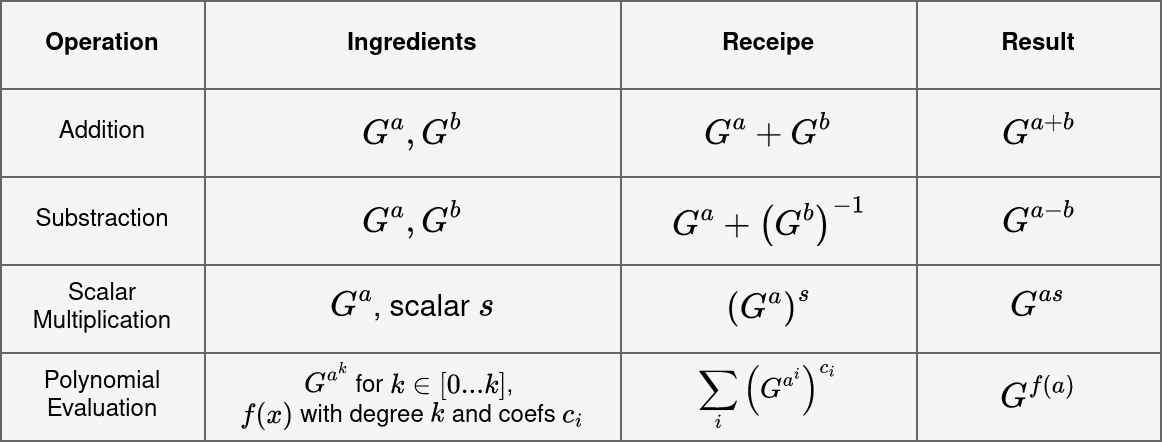
\includegraphics[width=1\linewidth]{figures/ec_arithmetic.drawio.png}
    \caption{Arithmetic on elliptic curves} 
    \label{fig:ec-arithmetic}
\end{figure}

\hl{polynomial evaluation is MSM, describe something about it and explain that it is a big part of the plonk computaiton}
\hl{maybe describe the Pipenger approach}

You should be familiar with the first two. The third one is just a generalization of exponentiation. And it would be unfair of us to leave the last without an explanation.

Any polynomial $f(x)$ of degree $k$ can be written in form $f(x) = c_0 + c_1 x + c_2 x^2 + c_3 x^3 + ... + x^k$. That means evaluation of $f(x)$ at some point $a$ can be written as $$G^{f(a)} = G^{c_0 + c_1 a + c_2 a^2 + c_3 a^3 + ... + a^k}$$
This can be split into terms as:$$G^{c_0 + c_1 a + c_2 a^2 + c_3 a^3 + ... + a^k} = G^{c_0} + G^{c_1 a} + G^{c_2 a^2} + G^{c_3 a^3} + ... + G^{a^k} = \sum_{i=0}^k (G^{a_i})^{c_i}$$

The arithmetic operations directly follow from description of the group. We would definitely want to calculate addition and multiplication, with corresponding inverses. Moreover besides point multiplication scalar multiplication will be also useful. Operation which will be particularly useful is a multi-scalar multiplication MSM in form $a_1g_1 + a_2g_2 + ... a_ng_n$ where $g$ are group elements and $a$ are scalars. As will later turn out this operation dominates the prover costs and it is a significant bottleneck. The complexity of the operations is greatly dependant on the bit length $b$ of the chosen group $\mathbb{G}$. In other words it is the number of bits needed to represent arbitrary element of a group.

\hl{Homomorphic encryption}
% \subsection{Homomorphic Encryption (inspiration how snarks work)}
% Remember the problem from example 2? Now we have all the tools to improve this protocol. We will use encryption function $E(r) = g^r$ where $g$ is a generator of elliptic curve group. Encrypting polynomial evaluated in $r$ with coefficients $c_i$ could be done as $E(r^i)^{c_i} = g^{r^i c_i}$. Evaluation of a polynomial will be denoted as: $E(p(r)) = g^{p(r)} =  (g^1)^{c_0} \cdot (g^{r^1})^{c_1} \cdot (g^{r^2})^{c_2} \cdot \ldots \cdot (g^{r^d})^{c_d}$. In order to make this more clear let's look at a specific example. Say we would like the prover to evaluate polynomial $p(x) = x^3 - 3x^2 +3x$ on the point $r$ without directly revealing $r$. Fist we need to encrypt values $E(r^3), E(r^2), E(r)$ which will be sent to prover. He can then reconstruct the polynomial as follows:

% $$E(r^3)^1 \cdot E(r^2)^{-3} \cdot E(r^3)^2$$
% $$g^{(r^3)^1} \cdot g^{(r^2)^{-3}} \cdot g^{(r^3)^2}$$
% $$g^{r^3 - 3r^2 + 2r}$$


% Given values $E(r^3), E(r^2), E(r)$ can now calculate evaluations $g^{p(r)}, g^{h(r)}$ in the encrypted space. The verifier will also validate the result in encrypted space by checking is $g^{p(r)} = g^{h(r)}g^{t(r)}$. These conditions make life of a dishonest prover much harder, because now he does not know much about the secretly sampled value $r$. % % \hl{more rigorou explanation for why it is harder}
% We have now greatly limited the possibilities of cheating the protocol is still not sound. 

% Remember that there was also a third point, which said that there is nothing constraining the prover to using polynomial of a different degree. Although we have restricted the prover in selection of powers of $r$ we have not restricted him to using them. That is why the verifier need a prove that only the supplied encryption were used to calculate $g^{p(r)}, g^{t(r)}$ and nothing else.


\subsection{Elliptic curve pairing}
Pairings are in essence deterministic mapping to another group. To be more specific it is a bilinear mapping that takes two encrypted elements $g^a, g^b$ of same (source) group and combines them by multiplication into an element of another (target) group, formally: $e(g^a, g^b) = e(g, g)^{ab}$. As you would have probably guessed it is not possible to multiply values from the target group and source group unless extreme cases such that $a = b = 1$. Also this operation is not reversible in polynomial time. % % \hl{why} Good analogy to think about this concept is that the result of a pairing is expressed under different generator.

The core properties for our purposes can be presented as:
$$e(g^a, g^b) = e(g^b, g^a) = e(g^{ab}, g^1) = e(g^1, g^{ab}) = e(g^1, g^a)^b = e(g^1, g^1)^{ab}$$

% % \hl{add this}
\begin{enumerate}
    \item not all groups where DLP is hard are pairing-fiendly
    \item pairing friendly  goups are usually slower to compute
    \item embeding degree
    \item multiplicative homomorphism but only for a single multiplication
\end{enumerate}


% ==============================================================================
% ===POLYNOMIALS================================================================
% ==============================================================================
\section{Polynomials toolkit}

\subsection{Comparing polynomials}
We will commonly test if some polynomials are equal just by comparing them at a single uniformly randomly chosen point. At first sight, this seems like the dumbest most naive approach, however, for a large enough domain, it works pretty well. 

\begin{theorem}{Intersection of polynomials} \newline
\label{theorem:poly-intersection}
    Arbitrary two polynomials in form $a_0 + a_1x + a_2x^2 ... a_nx^n = 0; b_0 + b_1x + b_2x^2 ... b_m x^m = 0$ where both $n, m \leq d \in \mathbb{N}$ intersect in no more than $d$ points.
\end{theorem}

\begin{dukaz} \newline
    To find the intersection points we need to solve equation $a_0 + a_1x + a_2x^2 ... a_nx^n = b_0 + b_1x + b_2x^2 ... b_m x^m$ which will produce yet another polynomial of degree $max(n,m) \leq d$. From the Fundamental Theorem of Algebra we know that a polynomial of degree $d$ cannot have more than $d$ roots.
\end{dukaz}

Now we want to check that $p = q$. If the polynomials are indeed equal then for sure $\forall x: p(x) = q(x)$. However, if they differ we can calculate the failure rate of this approach. The polynomial might intersect in almost $d$ points, so the probability of randomly selecting one of the intersection points is $\frac{d}{\text{domain size}} = \frac{d}{|\field|}$. This probability is usually considered negligible since the order tends to get really big. For example, the mentioned group $BLS12-381$ has order $\approx 2^{381}$. In a nutshell, we can effectively compare polynomials just by a single evaluation since the failure rate is small enough for most of the practical scenarios.

This observation turns out to be very useful and is commonly used in probabilistic approaches. The multivariate version (for polynomials of more variables) it goes by the name \href{https://en.wikipedia.org/wiki/Schwartz%E2%80%93Zippel_lemma}{Schwartz-Zippel lemma}.


\subsection{Interpolation}
\subsection{Lagrange interpolation}
\begin{definition}[Lagrange basis]
    The Lagrange basis is defined as:
    $$
    L_i(x) = 
        \begin{cases} 
            1 & x = 1 \\
            0 & \text{otherwise}
       \end{cases}
    $$
    A function that achieves this property is: $L_i(x) = \prod_{k \in [n], k \neq i} \frac{x-k}{i-k}$
\end{definition}

Lagrange interpolation is a method used in numerical analysis to approximate a function that passes through a given set of points. Given a set of data points $(x_i, y_i)$, where $x_i$ and $y_i$ are the independent and dependent variables, respectively, Lagrange interpolation constructs a polynomial that passes through all these points.

\begin{lemma}
    Univariate Lagrange Interpolation: let $p$ be a prime larger than $n$ and $\mathbb{F}_p$ field. For any vector $a = (a_0, ..., a_{n-1}) \in \mathbb{F}_p^n$ there is a unique univariate polynomial $q_a$ of degree at most $n-1$ such that: $\forall i \in [n-1]: q_a(i) = a_{i+1}$.
\end{lemma}

We will not go over the proof instead try to explain how it will be used in the protocol. For readers suspicious of this claim the proof could be found on page 18 of \cite{ProofArgsAndZk}. The Lagrange interpolation is carried by so called Lagrange basis $L_i(x)$. This is an expression that evaluates to 1 only for input $i$ and 0 otherwise. This means we are able to interpolate $a$ into a unique polynomial:
$$q_a(x) = \sum_{i=0}^{n-1} a_i L_i(x)$$

If you are curious about how this basis looks it is defined as:

\begin{definition}
    Lagrange basis: $$L_i(x) = \prod_{k \in [n-1], k \neq i} \frac{x-k}{i-k}$$
\end{definition}

Properties of this polynomials are easy to observe. When $x \in [n-1] \setminus i$ is plugged into $L_i(x)$ then then there will be exactly one fraction $\frac{x-k}{i-k}$ for which $k = x$ and that would make the product 0. If $x = i$ the consequence is even more trivial because all of the fractions would result in $\frac{i-k}{i-k} = 1$ and since $k \neq i$ everything simply results to 1. In the plonk paper it is represented as $L_i(x) = \frac{c_i(x^n-1)}{x-i}$ do not yet see why.

\begin{definition}[n-th root of unity]
    Generally, $n$-th root of unity is a number $\omega$ where $n$ is positive integer and $\omega^n = 1$. In this case we will be dealing with $\omega$ specifically picked from $\field$
\end{definition}


\subsection{Vanishing polynomial}
$$H = \{\omega, \omega^2, \omega^3, \ldots, \omega^{n}\}$$

\begin{lemma}{Sparse Vanishing Polynomial}
    \label{lemma:vanishing-poly}
    with domain $H$ can be represented in a sparse way
\end{lemma}

\subsection{Polynomial Division}

%%%  ===========================================================================
%%%  ===ARITHMETIZATION=========================================================
\section{Arithmetization}
\label{chap:arithmetization}

\subsection{Compilation}
Before we can think about arithmetization of some circuit it would be nice to first mention where this circuit came from. It is best to think of this as a computer program, where in order to run some high-level language the code first needs to be compiled into machine instructions. I will sweep the details under the rug but the point is the program is then executed in the processor, which has dedicated circuits for performing the necessary operations. We can express any complex computation in the form of some circuit. Some of the project for writing a ZK programs and compiling them into circuits are Circom or Noir from aztec. 

\subsection{Gate equations}
As in every other $\plonk$ explainer, we will also show the process of arithmetization on an example circuit. Consider a circuit for computing $(x_1 + x_2)(x_2s_1)$ where $x$ are public inputs and $s$ is a secret number, which only the prover knows. Since we know that there are at most binary gates, we can think of each gate as a row of a table, where columns are in order: left input, right input, and gate output. Look at the diagram below \eqref{fig:toy-circuit} on the first row. The $gate_0$ has left input $x_1$, right input $x_2$ and output $x_1 + x_2$. 

\begin{figure}[H]
    \centering
    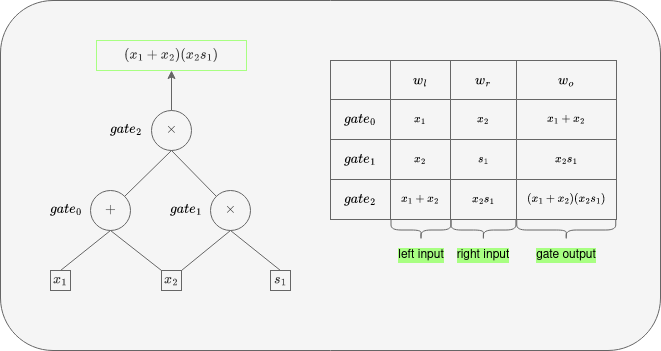
\includegraphics[width=1\linewidth]{figures/arithmetization.drawio.png}
    \caption{Toy Circuit}
    \label{fig:toy-circuit}
\end{figure}

Remember that the objective is to efficiently encode an arithmetic circuit into a set of polynomials. The first step will be to encode each gate as an equation. Later in the \hyperref[chap:round0]{setup phase}, we will combine these equations into polynomials via interpolation. Considering only gates for addition and multiplication each gate could be written as one of the following:

\begin{align}
    \label{eq:primitive_gate_constraints}
    \text{\textit{addition:} } \text{left input} + \text{right input} = \text{gate output} 
    \\
    \text{\textit{multiplication:} } \text{left input} \times \text{right input} = \text{gate output}
\end{align}

That is a good start, but it would be even nicer if we could create an equation that can check the validity of both gate types. Notice that each column of computation table \eqref{fig:toy-circuit} could be also viewed as a vector. By assigning $x_1 = 2, x_2 = 1, s_1 = 3$ we would get vectors $w_l = [2, 1, 3], w_r = [1, 3, 3], w_o = [3, 3, 9]$. These numbers represent the whole computation of the program and in the context of $\plonk$, they are referred to as the witness. So, in the end, witness are just vectors of a bunch of numbers. Notice that all of the vector has length 3 which is the number of gates in the circuit. For the rest of the posts, we will denote $n$ as the number of gates in the circuit.

Besides, we also need something to specify the type of the gate and this is done by selectors: $q_l$ left, $q_r$ right, $q_o$ output, $q_m$ multiplication, $q_c$ constant. Again nothing scary, these will be vectors of size $n$ \textit{selecting} the type of gate which we want to use. For example, if we are dealing with gate $i$ that is a multiplication gate then $q_{m_i} = 1$ otherwise it is always set to 0.
Now we will introduce an extended equation for gate number $i$. This equation makes sure that each of the gates is computed correctly. To verify the multiplication gate we need: $w_{l_i}w_{r_i} = w_{o_i}$ and to verify the addition gate $w_{l_i}+w_{r_i} = w_{o_i}$. We will combine these two and show how to assign the selector to pick the type of gate we want to use.

\begin{figure}
    \centering
    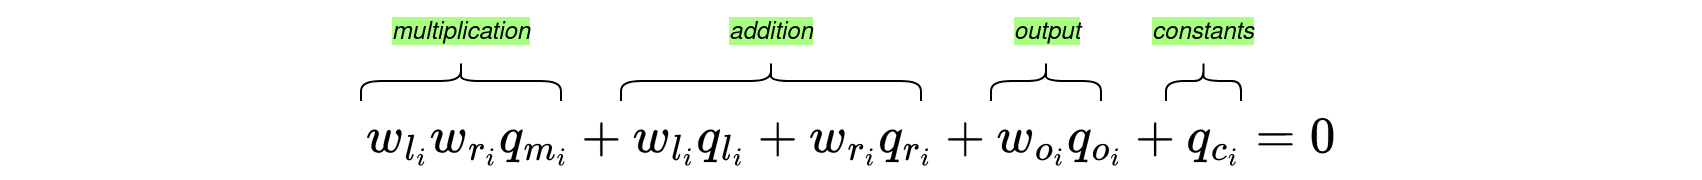
\includegraphics[width=1\linewidth]{figures/gate_equation.drawio.png}
\end{figure}

Consider the example circuit and variable assignment $x_1 = 2, x_2 = 1, s_1 = 3$, and for simplicity, all unassigned selectors will have value 0. Then it is possible to perform these operations:


\begin{itemize}
    \item \textit{addition:} $q_{l_i} = q_{r_i} = 1, q_{o_i} = -1$
        
        For the addition gate, want to keep only the addition and output terms of the equation the rest will cancel out thanks to the remaining selectors being 0. Let's illustrate it on an example circuit and construct the equation for an addition gate $gate_0$:
        $$2\cdot 1 \cdot 0 + 2 \cdot 1 + 1 \cdot 1 + -1 \cdot 3 + 0 = 0$$
        $$2 + 1  -3 = 0$$
        $$2 + 1 = 3$$
    \item \textit{multiplication:} $q_{m_i} = 1, q_{o_i} = -1$

        To engage a multiplication gate we assign the selector such that only the multiplication and output terms of the equation remain. Below is the gate equation for multiplication gate $gate_1$:
        $$1 \cdot 3 \cdot 1 + 1 \cdot 0 + 3 \cdot 0 + -1 \cdot 3 + 0 = 0$$
        $$1 \cdot 3 -3 = 0$$
        $$1 \cdot 3 = 3$$
    \item \textit{constant assignment:}
        
        Besides the operations of addition and multiplication, it is possible to do constant assignments (not illustrated on the example circuit). Say that we want the left input of a $gate_i$ to be equal to some constant $c$. To construct the equation for this gate we can assign $q_{l_i} = 1, q_{c_i} = -c$, and the equation then simplifies to $w_{l_i} = c$, checking exactly what we want. This work respectively also for the right input we just set the selectors as $q_{r_i} = 1, q_{c_i} = -c$.
\end{itemize}


Notice that using the selector polynomial some terms are canceled out so that we get to the separate gate constraints described in the beginning \eqref{eq:primitive_gate_constraints}. To better see how the selectors should be assigned for the example circuit check the diagram below.

\begin{figure}[H]
    \centering
    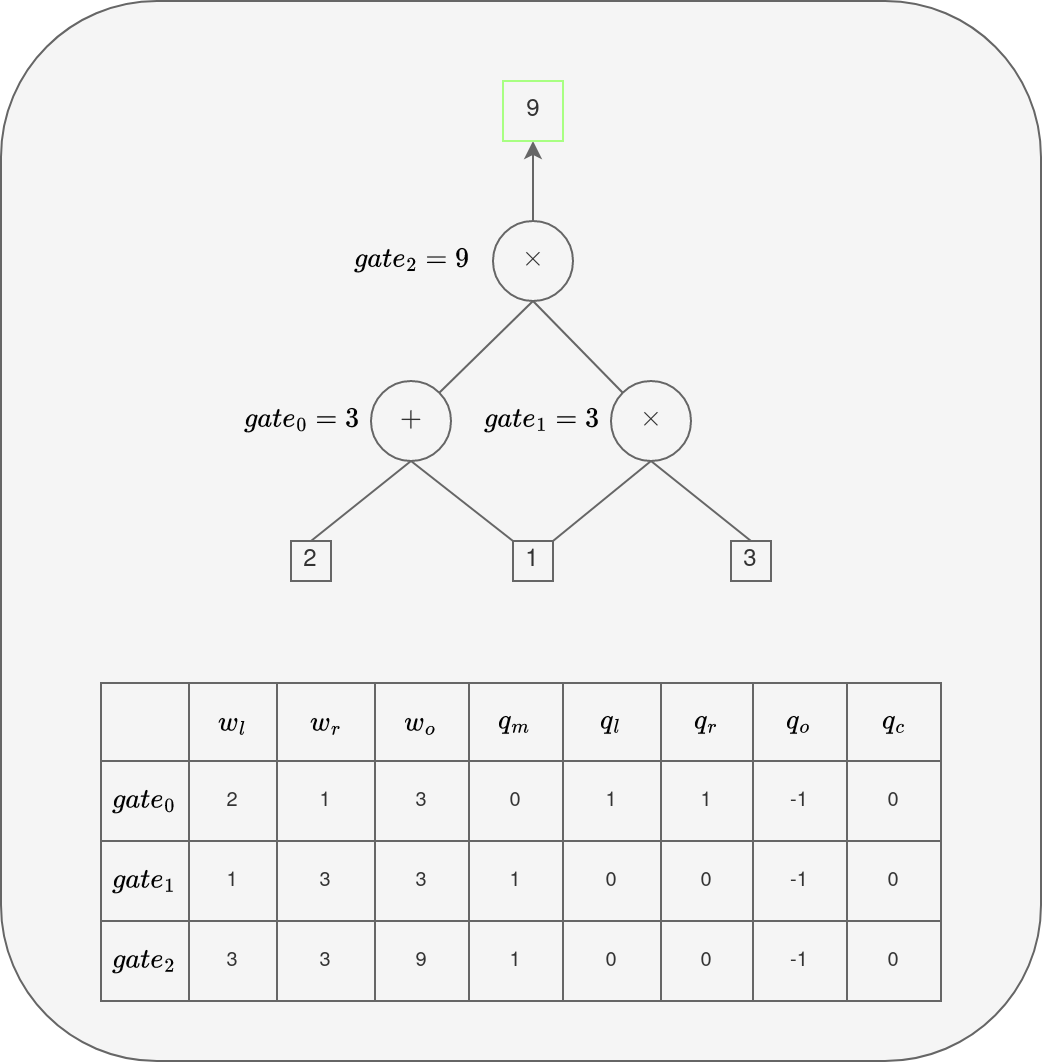
\includegraphics[width=0.75\linewidth]{figures/arithmetization_evaluated.drawio.png}
    \caption{Evaluated diagram}
    \label{fig:evaluated-circuit}
\end{figure}


Now we can get a bit closer to the arithmetization that is used in $\plonk$ we merge the witness vector $w_l, w_r, w_o$ into single $w$ such that: $$w_l = [w_0, \dots, w_{n-1}], w_r = [w_n, \dots, w_{2n-1}], w_o = [w_{2n}, \dots, w_{3n-1}]$$ 
Now the witness $w$ encapsulates all of the values flowing through the circuit, where some of the values are public and some are secret. The verifier needs to check the output of the circuit and the public input, so naturally, these two will be public. The rest of the values remain private.

To get the full gate equation we add one last thing. The public input to the circuit will be denoted by vector $PI$, remember that public input is a subset of the witness. In contrast to selector $q_c$, $PI$ can be changed for each execution of the circuit while 
$q_c$ constants (surprisingly) remain bound to a specific circuit. For all (inner) nodes not related to input $PI$ will be set to 0. The full $\plonk$ gate equation looks like this:
\begin{equation}\label{gate-constraint}
    w_{i}w_{n+i}q_{m_i} + w_{i}q_{l_i} + w_{n+i}q_{r_i} + w_{2n+i}q_{o_i} + PI_i + q_{c_i} = 0 
\end{equation}

Let's revise this on our beloved Sudoku game. Imagine the prover is trying to convince the verifier that he knows the solution to a \href{https://en.wikipedia.org/wiki/Sudoku}{Sudoku problem}. Then the circuit is a program that checks if the Sudoku is filled validly and the prover wants to show that he can fill in such numbers that this program accepts his solution. Here the public input (public part of the witness) could be the initial state of the Sudoku problem as well as the dimensions of the board. Naturally private witnesses are the numbers that need to be filled in the board that the prover claims to know and does not want to share. We should also mention that there is a convention that the correct result of the circuit should be 0. That is the same as saying the output of the program is 0 if it succeeds.


\subsection{Transcription into polynomials}
This section was inspired by the lecture of Dan Boneh which is available on \href{https://zkhack.dev/whiteboard/}{ZK Whiteboard}. Since in the group of elliptic point we had only operation with addition and multiplication these will also be the only gates that we will use. Subtraction and division will be simulated by computing additive and multiplicative inverses. It is possible to work also with custom gates but for the simplicity this will be discussed in another section. For now we will consider only 2 binary gates. 

Let's see how a specific circuit can be transformed into a polynomial. Take arithmetic operations $(x_1 + x_2)(x_2 + w_1)$ where $x$ are public inputs and $w$ is a secret witness. This can be visualized as a computation graph where the first sum is computed in addition $gate_0$, second sum in addition $gate_1$ and finally the product in $gate_2$.

% \begin{table}[ht]
%     \centering
%     \begin{tabular}{ l | l l l}
%      inputs:   & $x_1$ & $x_2$ & $w_1$       \\ 
%      \hline
%      $gate_0$: & $x_1$ & $x_2$ & $x_1 + x_2$ \\ 
%      $gate_1$: & $x_2$ & $w_1$ & $x_2 + w_1$ \\ 
%      $gate_2$: & $x_1 + x_2$ & $x_2 + w_1$ & $(x_1 + x_2)(x_2 + w_1)$ \\
%     \end{tabular}
%     \caption{Arithmetic circuit as a table}
% \end{table}

Notice how the first two columns show input and the third one output. The number in the right corner is 77 which is output of the arithmetic circuit. We set notation $|C|$ as number of gates in $C$, and also $|I| = |I_x| + |I_w|$ as number of public inputs plus number of private inputs. For case of binary gates the total number of elements in the computation trace is $d = 3|C| + |I|$ and we will also have set $\Omega = \{1, \omega, \omega^2, ..., \omega^{d-1} \}$. Now we are able to specify polynomial which partially represents the table. 

In the original paper the each gate $i$ could be represented by a equation:

$$q_{l_i} a_i + q_{r_i} b_i+ q_{o_i} c_i + q_{m_i} a_i b_i + q_{c_i} = 0$$

where $a, b, c$ are left right and output wires and $q$ are selector polynomials. Specifically $q_l, q_r, q_o, q_m, q_c$ stand for left right output multiplication and constant, these are called selector and specify encode the structure of the circuit . Now for each gate we can perform three operations:
\begin{itemize}
    \item addition: by assigning 1 to selectors $q_l, q_r$, -1 to $q_o$ and 0 to remaining  
    $a + b = c$
    \item multiplication: by assigning 1 to $q_m$, -1 to $q_o$ and 0 to remaining $a \times b = c$
    \item constant assignment: is done when binding to some public variable. we can bind it to the left variable by assigning $q_l = 1$, $q_c$ value we want to assign and rest is zero. $b = q_c$
\end{itemize}

% \begin{definition}
%     Polynomial representing computation trace is $t \in \mathbb{F}_{p}^{\leq d}$ such that it encodes all inputs as $t(\omega^{-j})$ for $j \in [|I|]$ and all wires $\forall l \in [|C|-1]$ in following manner
%     \begin{enumerate}
%         \item $t(w^{3l})$ is left input to gate $l$
%         \item $t(w^{3l+1})$ is right input to gate $l$
%         \item $t(w^{3l+2})$ is output of gate $l$
%     \end{enumerate}
% \end{definition}

% If we take the previous example we now have define polynomial in its evaluation form with degree $d-1$:

\begin{table}[h]
    \centering
    \begin{tabular}{ l | l l l}
     inputs:   & $t(\omega^{-1})= x_1$ & $t(\omega^{-2})=x_2$ & $t(\omega^{-3})=w_1$ \\ 
     \hline
     $gate_0$: & $t(\omega^{0})=x_1$  & $t(\omega^{1})=x_2$  & $t(\omega^{2})=x_1 + x_2$ \\ 
     $gate_1$: & $t(\omega^{3})=x_2$  & $t(\omega^{4})=w_1$  & $t(\omega^{5})=x_2 + w_1$  \\ 
     $gate_2$: & $t(\omega^{6})=x_1 + x_2$ & $t(\omega^{7})=x_2 + w_1$  & $t(\omega^{8})=(x_1 + w_2)(x_2 + w_1)$ 
    \end{tabular}
    \caption{Arithmetic circuit as a table}
\end{table}

% Now the polynomial will be interpolated. For example with FFT in time $d \log_2{d}$. This encoding has one flaw, can you spot it? We are not able to distinguish types of the polynomials and that is why we need selector polynomial. 

% \begin{definition}{Selector polynomial}
%     $s(x) \in \mathbb{F}_p^{\leq d}(x)$ such that $\forall l \in [|C|-1]$:
%     $$
%     s(x) = 
%     \begin{cases} 
%         s(\omega^{3l}) = 1 & \text{if gate is for addition}\\
%         s(\omega^{3l}) = 0 & \text{if gate is for multiplication}
%       % $0 & x\leq 0$ \
%    \end{cases}
%    $$
% \end{definition}
% Notice that this polynomial does not depend on the inputs, so could be precomputed during the setup phase. To encode the circuit correctly the following needs to hold $\forall x \in H_{gates} = \{1, \omega^3, \omega^6, ... \omega^3{|C| -1},\}$:
% $$s(x)(p(x) + p(x\omega)) + (1 - s(x))(p(x)p(x\omega)) = p(x\omega^2)$$

% I understand that this might look intimidating at first glance but actually the equation is very straight forward. For each gate we are now able to specify the type. If it is addition then the output of this gate would be $p(x) + p(x\omega)$ and otherwise $p(x)p(x\omega)$.

% ----------------------------------------------

To make this more succinct it would be nice to represent the whole circuit as a single polynomial. The key point to realize here is that system of equations in the same form could be interpreted as a single equation over polynomials. Suppose we have a vector like $v=(5,8,13)$. We can convert the vector into a list of points $(0,5),(1,8),(2,13)$ simply using the index of the value in the vector as the x-coordinate. Then there is a unique degree-2 polynomial function that passes through these points. Notice that we are entirely free to choose any domain we want. In $\plonk$ the polynomials are interpolated over the domain of roots of unity. The $n$-th root of unity is simply a group element that satisfies $x^n = 1$ and for $i<n, x^i \neq 1$. Let's have a set $\Omega = \{1, \omega, \omega^2, \omega^3 ..., \omega^n-1\}$

To make this complete we need to realize that gate wire constraints $a, b, c$ are different for each of the equation and we can just transform them to polynomial to arrive to:
$$L(x)a(x) + R(x)b(x) + O(x)c(x) + M(x)a(x)b(x) + O(x) + C(x) = 0$$


By transcribing the problem we are reinterpreting the problem in terms of polynomial. We are asking the prover to give us witness $w$ such that together with the public input $x$ a specific program encoded circuit $C$ will give out some value. In the general case we are asking for such $w$ that $C(x,w) = 0$. Right now we will consider gates just with standard group operations. By that we mean addition and multiplication. In later sections we will see that it is also possible to construct $\plonk$ with custom gates, for now we will make our life easier by dealing only with binary gates.

During the process of arithmetization the the $\mathcal{V}$ needs to make sure that $\mathcal{P}$ did not cheat in any way. In particular we need to have gate constraints, which are equations between wires that are attached in the same gate. Secondly we will also want to have copy constraints that guarantee that for two consecutive gates the output of the first one is input to the second one. 

%%%  ===========================================================================
%%%  ===COMMITMENT SCHEME=======================================================
\section{Commitment Scheme}
Commitment scheme is a long studied cryptographic primitive. It's a way of securely committing to a piece of data, ensuring that it remains unchanged throughout the process of verification. Motivation of this mechanism is to prevent the prover from generating proof depending on the query from verifier. By committing to some value, he will not be able to change it afterwards. This mechanism by definition needs to be binding and hiding. Loosely speaking these notions mean that after commitment the values cannot be changed by the committer and the real value remains hidden for the verifier. If you would insist on a metaphor we could imagine that that the committer locks his precious information into a container and gives it to the verifier. After this point the committer does not have access to it and, thus cannot change it anymore. Moreover, since the box is locked the verifier cannot look into it but can ask the committer to unlock only a small part of it which would be just enough for verification of the information. In this section we will be referring to the committer and prover interchangeably since the role of committer is taken only by the prover and the verifier just remains verifier.

To get back to the context of this article, we will be talking about polynomial commitment schemes. The information the committer or rather prover has of knowledge is a polynomial $q$, because the letter $p$ is already overloaded. We also need to keep in mind that the degree of this polynomial is bounded by specified $d$. Point of the scheme is to convince the verifier of knowledge of the coefficients of $q$ without giving them away. A standard polynomial commitment scheme should have these procedures:
\begin{enumerate}
    \item $commit$: make $\mathcal{P}$ "stick to" polynomial $q$.
    \item $open$: $\mathcal{V}$ challenges $\mathcal{P}$ to evaluate $q$ at random point $r$
    \item $verity$: $\mathcal{V}$ receives the evaluations and performs checks to decided if it is valid
\end{enumerate}

\procedureblock{Polynomial Commitment Scheme}{%
    \textbf{Committer} \>\> \textbf{Verifier} \pclb
    \pcintertext[dotted]{Setup ceremony}
    \text{send commitment} \> \> \\
    \> \sendmessageright*{[q]_1} \> \\
    \> \> z \sample \field \\
    \> \sendmessageleft*{z} \> \\
    \text{evaluate}
    \> \sendmessageright*{q(z)} \> \\
    \>\> \text{verify}
}


The commitment is a single evaluation of $q$ and in the opening phase the verifier asks for another evaluation at a random point $r$. After $q(r)$ is sent by the prover verifier is able to tell with non-negligible probability if the prover is right. In particular the motivation behind this concept is that the prover would not be able to choose $q$ depending on the query $r$ without breaking the computational assumptions. To be more specific about the properties of the commitment I need to explain what binding and hiding formally means.

\begin{definition}{Binding property}
    guarantees that that for a polynomial commitment scheme there is polynomial $q$ of appropriate degree such that evaluation queries on $q$ correspond to answers provided by the committer to the verifier. 
\end{definition}

\begin{definition}{Hiding property}
    suggest that for polynomial $q(x)$ and its commitment $c$ and any efficient $\mathcal{A}$ a randomly chosen polynomial $r(x)$ with the same degree is computationally indistinguishable from $q(x)$.
\end{definition}

By itself these properties are useful but for purposes of our protocol there are not sufficient. Can you spot the problem? The binding property says that there is exists a polynomial of appropriate degree which can pass the verification check, however we also need to make sure that the prover is not cheating and he possess the knowledge of $q(x)$. Another notion we will formalize will make sure that if the verifier can answer the queries successfully than he needs to have knowledge of the committed polynomial.

\begin{definition}{Extractable scheme}
    guarantees that $\forall$ efficient committers $\mathcal{A}$ that take as input public parameters with degree bound $d$ and output commitment $c$ $\exists$ efficient extractor algorithm $E$ that has the same input as $\mathcal{A}$ and produces polynomial $q$ in degree bound $d$ such that evaluation queries on $q$ correspond to answers of $\mathcal{A}$ to these queries.
\end{definition}

This definition at first seems a bit cryptic but all that it is trying to say is that that $\mathcal{A}$ needs to have knowledge of $q$. That follows from the fact that $E$ is efficient and therefore an efficient $\mathcal{A}$ can afford to run it. Since $E$ does not anything more than $\mathcal{A}$ and can produce $q$ that can use $E$ to get knowledge of $q$ which passes all queries.

There are numerous different approaches to design polynomial commitment schemes. We will be specifically interested in KZG since that is the one that was used in the original plonk paper. The following section and proof were taken from \cite{ProofArgsAndZk}. 

\subsection{KZG commitment scheme}
Before we proceed any further we need to mention the structured reference string SRS which is a part of one-time setup procedure of $\plonk$. This information will be public for any party and its knowledge is needed for anyone who will want to make a commitment. SRS consist of evaluations $\{g, g^{\omega}, g^{\omega^2}, ..., g^{\omega^{d-1}}, g^{\omega^{d}}\}$ where $d$ is degree bound and and $\omega$ is uniformly randomly chosen $\omega \in [p-1]$. The number omega is commonly referred to as "toxic waste" in other articles. That is because this value is indeed very dangerous and is fallen into the evil hands of adversary the commitment could be faked. I cannot stress this enough, after the setup delete you omegas burned them down as soon as SRS is generated otherwise all of the effort would come in vain. Here is what we would need for KZG, these information will be public:
\begin{enumerate}
    \item $e$: is a symmetric bilinear map meaning in $\mathbb{G}_1 \times \mathbb{G}_2 \rightarrow \mathbb{G}'$ the groups $\mathbb{G}_1$ and $\mathbb{G}_2$ are equal.
    \item $\mathbb{G}, \mathbb{G}'$ are pairing friendly groups both under the field  $\mathcal{F}_p$ for $p$ prime
    \item $g$ is a generator of the group
    \item $d$ is the upper bound on the polynomial degree
    \item SRS evaluations $\{g, g^{\omega}, ... ,g^{\omega^d}\}$
\end{enumerate}

As we will late see both commitment and opening contain only constant number of group elements, which makes this scheme fast. We will now proceed to a construction of imperfect KZG scheme which is non-extractable and that modify it to fix this flaw. Let's start by a simple lemma:

\begin{lemma}
    For any $d$-degree univariate polynomial $q \in \mathbb{F}_p$ the assertion $q(z) = v$ is equivalent to checking if there exists polynomial $w(x)$ under the same field of degree at most $d - 1$ such that: $w(x) = \frac{q(x)-v}{x-z}$
\end{lemma}

\begin{dukaz}
    To prove $q(z) = v$ implies existence of $w(x)$ we simply plug $z$ into $q(x)-v = w(x)(x-z)$ which results into $0 = w(x)0$. This is satisfied for an arbitrate polynomial. Other way around we have $w(x) = \frac{q(x) -v}{x-z}$ and want to show that $q(z) = v$. By looking just at $q(x)-v = w(x)(x-z)$ we could notice that if we shift the polynomial $q(x)$ down by $v$ then it has root at point $z$. For a polynomial $r(x) = q(x) - v$ the evaluation of $r(z) = 0$. In each evaluation the values of $r$ and $q$ differ by $v$. So if we know that $r(z) = 0$ then it must follow that $q(z) = v$, which is what we wanted to achieve.
\end{dukaz}

\subsubsection{Commitment}
To commit to $q$ over $\mathbb{F}_p$ the committer $\mathcal{P}$ sends $c$ which he claims is equal to $g^{q(\omega)}$. How does he calculate the evaluation without knowing $\omega$? Recall from the section about polynomials that: $q(x) = \sum_{i=0}^{d} c_i x^i \rightarrow g^{q(\omega)} = \prod_{i=1}^d (g^{\omega^i})^{c_i}$ for $\{c_0, ... , c_d\}$ which are the coefficients of $q$.

\subsubsection{Opening}
To open at input $z \in [p-1]$ for a value $v$ meaning that $q(z) = v$ the committer needs to compute witness polynomial.
$$w(x) = \frac{q(x)-v}{x-z}$$

% % \hl{nice observation $q(x) - q(z)$ has one obvious root which is $z$ $\rightarrow$ if i get $q(z)$ there must exist $w(x)$}

Then he will evaluate at $g^{w(\omega)}$ which is possible to calculate without knowledge of $\omega$ using same approach as in the commitment. Assuming $\mathcal{P}$ has knowledge he will evaluate also $q(z) = v$ and send pair $(v, g^{w(\omega)})$to $\mathcal{V}$. It is important to note that $z \neq \omega$, however we do not need to worry about it. With commonly used prime field there is only a very negligible probability of randomly picking $z = \omega$.

\subsubsection{Verification}
The verifier has knowledge of $c, v, g^{w(\omega)}$ provided by the prover, $z$ generated by himself and SRS which is public for all parties. The only check that needs to be done by the $\mathcal{V}$ is:
$$e(cg^{-v}, g) = e(g^{w(\omega)}, g^{\omega} g^{-z})$$
Note that from the whole SRS only $(g, g^\omega)$ are needed for the evaluation which is why in many works SRS is referred to as prover key and $(g, g^\omega)$ as a verification key. 

There are quite many variable in the play and lot of things going on. To make it a bit more clear let's expand the expression from the verification.
$$e(g^{w(\omega)}, g^{\omega} g^{-z}) = e(g^{\frac{q(\omega) -v}{\omega -z}}, g^{\omega -z}) = e(g, g)^{q(\omega) -v} = e(g^{q(\omega)-v} g, g) = e(c g^{-v}, g)$$

The last step of this expansion will be true if and only if $c = g^{q(\omega)}$. For a hones committer who knows $q$ the verification procedure would accept with probability 1, which shows correctness of the protocol. If the mechanism of the scheme feels still a bit blurry give this visualization of the communication might help you. 

\begin{figure}[H]
    \centering
    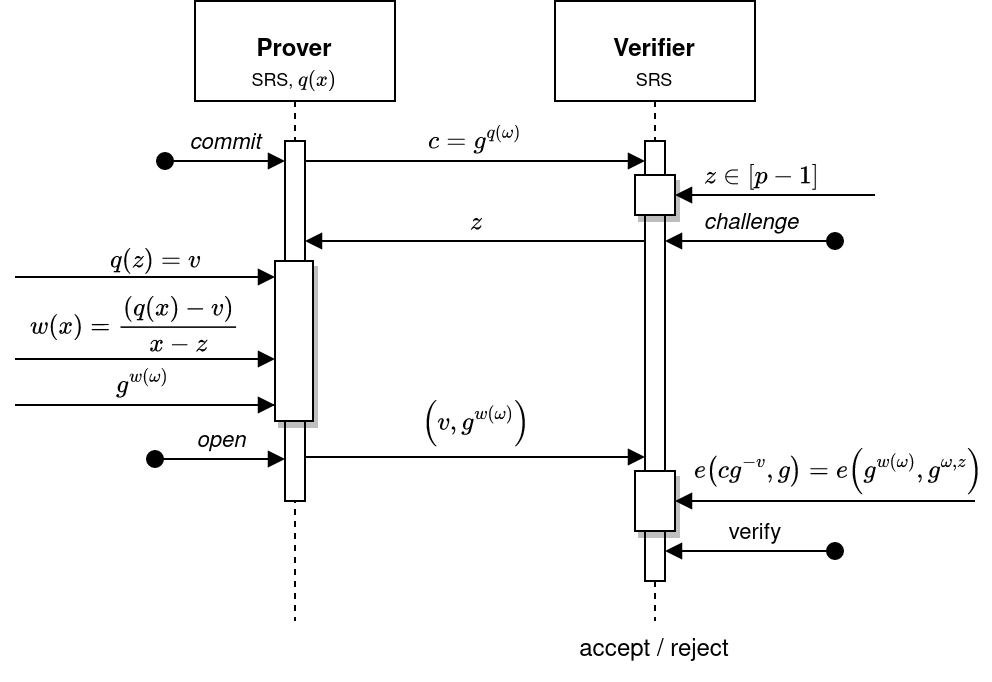
\includegraphics[width=\textwidth]{figures/kzg_diagram.png}
    \caption{Non-Extractable KZG PCS}
\end{figure}

Why all of the hassle with curve pairing, what is it used for? A mindful reader might have noticed that otherwise the verifier would not be able to perform the check. In detail the left side $g^{q(w) - v} = g^{q(w)} g^{-v}$ is easily computable, since $\mathcal{V}$ gets $g^{q(w)}$ can find exponentiate $g^v$ and then take the negative. Problem is with the right side where $\mathcal{V}$ has $g^{w(\omega)}, g^\omega, z$, thus can compute $g^{\omega - z}$, however $g^{w(\omega) (\omega - z)} = g^{w(\omega)^{(\omega - z)}}$. Remember that the value of $\omega$ is secret and should be destroyed immediately after setup, which means $\mathcal{V}$ has knowledge of $g^\omega$ but no $\omega$. This means he cannot calculate $(\omega - z)$ and thus is is not possible to compute $w(\omega) (\omega - z)$ in the exponent. Luckily this operation can be performed via curve pairing thanks to the property $e(g^a, g^b) = e(g, g)^{ab}$.

\subsection{KZG analysis}
\label{chap:kzg}

\subsubsection{Hiding}
This property is straight forward if we realize what the verifier gets. There is the commitment $c = g^{q(\omega)}$ which is one evaluation of the commitment polynomial and the real value is infeasible to extract due to DLP. Then as a part of verification $\mathcal{P}$ sends $g^{w(\omega)}$ which is likewise not possible to extract and single evaluation $q(z) = v$. After executing KZG commitment scheme $\mathcal{V}$ has two encrypted evaluations which reveal no information thanks to DLP and one plain text evaluation to the committed polynomial. To properly establish hiding property the polynomial $q$ has to be indistinguishable from a randomly chosen polynomial of the same degree. % % \hl{How to construct hiding game}

\subsubsection{Binding}
Binding property is a little harder to establish. First we introduce cryptographic assumption SDH

\begin{definition}{D-strong Diffie Hellman Assumption}
    SDH assumes that $\mathcal{P}$ given SRS has no efficient way of computing a pair $(z, g^{\frac{1}{\omega - z}})$ with non-negligible probability. 
\end{definition}

This assumption is stronger than DLP itself. We will show that this assumption needs to hold otherwise the $\mathcal{P}$ would be able to give two different witnesses for the same commitment which breaks the binding property.

\begin{lemma}
    Assuming SDH on KZG commitment the committer cannot can only open one valid value for request $v$.
\end{lemma}

\begin{dukaz}
    For a contradiction we can say that the $\mathcal{P}$ is able to open two different values $v \neq v'$. This would require calculating two different witness polynomials $w(\omega), w'(\omega)$:
    $$w(\omega) = \frac{q(\omega) - v}{\omega - z}, w'(\omega) = \frac{q(\omega) - v'}{\omega - z}$$
    Substracting them yields:
    $$w(\omega) - w'(\omega) = \frac{1}{\omega - z}  (v' - v)$$
    $$\frac{1}{\omega - z} = \frac{w(\omega) - w'(\omega)}{v' - v}$$

    Therefore, the $P$ would be able to calculate the division which leads to contradiction by violating the SDH assumption.
\end{dukaz}

\subsubsection{Extractable scheme}
We are almost satisfied with this PCS. As the last thing we need to prove that the scheme is extractable, so the prover needs to have knowledge of $q$. We would now need to modify the scheme by a bit. Now the SRS will be twice as long containing pairs $$\{(g, g^{\psi}), (g^{\omega}, g^{\omega \psi}), (g^{\omega^2}, g^{\omega^2 \psi}), ..., (g^{\omega^d}, g^{\omega^d \psi})\}$$. 

\begin{definition}{Power Knowledge of Exponent assumption (PKoE)}
    For any polynomial time $\mathcal{A}$ given access to SRS, whenever the algorithm outputs group elements $a, b \in \mathcal{G}$ such that $a = b^{\psi}$ then the $\mathcal{A}$ needs to know the coefficients that explain $a = \prod_{i=0}^d = g^{c_i \psi \omega^i}$. So $\forall \mathcal{A} \exists$ efficient algorithm $E$ that can produce the coefficients $c_i$.
\end{definition}

Essentially PKoE assumes that there is only one way of an polynomial time $\mathcal{A}$ can compute two group elements with such relation to each other. Now the commitment will be a pair $c = (g^{q(\omega)}, g^{q(\psi \omega)})$. The calculation of the witness polynomial remains the same and verifier needs to perform two checks:

$$e(g^{q(\omega)} g^{-v}, g) = e(g^{w(\omega)}, g^{\omega} g^{-z})$$
$$e(g^{q(\omega)}, g^\psi) = e(g^{q(\psi \omega)}, g)$$

To prove the extractability of the scheme we simply rely on the second verification check which simplifies to: $g^{q(\psi \omega)} = g^{\omega} g^{\psi}$. From the PKoE it needs to follow that $\mathcal{A}$ has knowledge of the coefficients therefor knows the polynomial $q$.

The completeness of this scheme holds for the same reason as before. And intuitively the scheme is still binding because the modification scheme only extends to one more verification checks but the first one already binds the commitment to a specific polynomial. 

\subsubsection{Time analysis}
To analyze the complexity of the final protocol we want to know how to KZG polynomial commitment scheme performs. The big advantage is that the commitment is constant in size because it is always just one group element. On the other hand $SRS$ is a lot bigger with $d$ elements from $\mathbb{G}_1$ and one element from $\mathbb{G}_2$. This requires significant computation but is done only once. Moreover, the prover requires only 2 elements from $SRS$. 

In the prover (committer) algorithm, there needs to be calculated commitment $C$ and witness $W$ and each requires a single MSM. Evaluation of $v$ can be done in constant time. Moreover to generate the witness the prover needs to do a polynomial division which is $O(n^2)$ in the common approach.

The verifier needs to compute $g^{-v}$ and also $g^z$ and two pairings. 1 $\mathbb{G}_1$ scalar multiplication, 1 $\mathbb{G}_2$ scalar multiplication and 2 pairings.

\subsection{Blinding}
So, far we have discussed the \hyperref[chap:kzg]{KZG commitment scheme} that is not zero-knowledge. Clearly, both commitment and openings reveal some information about the committed polynomial. Before we make our first commitment in the protocol we need to introduce some adjustments.

Committing plain polynomials by KZG is considered "safe" as KZG is computationally hiding. Even though the commitment effectively hides the polynomial, some information is revealed through the openings. In a common cryptographic setup it would not be a problem, however, remember that we are aiming to make the protocol zero-knowledge, so absolutely no information should leak. To achieve zero-knowledge, we will use blinding, by introducing randomness. $\plonk$ does this by mangling the former polynomial $p$ as follows: $$\Tilde{p}(x) = Z_H \times \text{some expression} + p(x)$$

Notice that the polynomials $p(x), \Tilde{p}(x)$ agree on all points of domain $H$ because $Z_H$ will evaluate to 0. In all of the proofs of the following rounds, we will be interested only in the domain $H$ and that is why it does not matter that $p(x), \Tilde{p}(x)$ might not match outside of $H$.

Consider that some polynomial $p(x)$ should be opened at challenge points $(z_1, z_2, ... z_{k})$ randomly chosen by the verifier. Then $\plonk$ suggests altering the committed polynomial with random blinding scalars $(b_1, b_2, \ldots, b_{k+1}) \in \field$ as: $$\Tilde{p}(x) = (b_1 + b_2x + b_3x^2 ... + b_{k+1}x^{k})Z_H(x) + p(x)$$

Notice that the degree of the blinding polynomial depends on $k$ the number of openings. Now the crucial question is, does $\Tilde{p}(x)$ reveal some information about $p(x)$? It does because for $\forall x \in H: p(x) = \Tilde{p}(x)$. However, the set $H$ is very small compared to the whole domain so the probability of randomly choosing an element of $H$ is negligible and we do not need to worry about it. Let's examine closer the case when $x \neq H$.

\begin{definition}{$k$-blinded polynomial}
    A polynomial $\Tilde{p}(x)$ is $k$-blinded form of $p(x)$ if constructed as
    $$\Tilde{p}(x) = b_k(x)Z_H(x) + p(x)$$
    where $b_k(x) = b_1 + b_2x + b_3x^2 \ldots + b_{k+1}x^{k}$ is a blinding polynomial with coefficients chosen independently and uniformly randomly and $Z_H(x)$ is polynomial vanishing on domain $H$.
\end{definition}


% \begin{definition}
%     A protocol $(\ldots)$ has $k$-wise zero-knowledge if there exists a probabilistic poly-time simulator $S$ such that for all interactive non-uniform polynomial time adversaries $\adv$

%     \[
%     \operatorname{Pr}
%     \left[
%     \begin{array}{c}
%         srs \gets \mathsf{Gen}(d) \\
%         c \gets \mathsf{Commit}(srs, q) \\
%         (z_1, z_2, ..., z_k) \gets \adv \\
%         (y, v_1, v_2, ..., v_k) \gets \mathsf{Eval}(srs, q, z)
%     \end{array}
%     :
%     \adv(c, (z_1, z_2, ..., z_k), (v_1, v_2, ..., v_k), g^{w(\tau)}) = 1
%     \right]
%     \]
    
%     \[
%     =\operatorname{Pr}
%     \left[
%     \begin{array}{c}
%         srs \gets \mathsf{Gen}(d) \\
%         (c, (v_1, v_2, ..., v_k), y) \gets \mathsf{Sim}(srs, (z_1, z_2, ..., z_k)) \\ 
%     \end{array}
%     :
%     \adv(c, (z_1, z_2, ..., z_k), (v_1, v_2, ..., v_k), y) = 1
%     \right]
%     \]
    
% \end{definition}


\begin{definition}{Honest verifier zero-knowledge (HVZK)}
    An interactive proof system $<\prover, \verifier>$ honest verifier zero-knowledge if there exists
    a probabilistic polynomial time simulator $\mathsf{Sim}$ with access to the verifier such that:
    $$\forall x \in \mathcal{L}: \mathsf{Sim}(x) \approx View_{V}(<\prover, \verifier>(x))$$
    
    Where $\mathsf{Sim}(x)$ and $View_{V}(<\prover, \verifier>(x))$ are distributions with the randomness of $\verifier$, and $View_{\verifier}(<\prover, \verifier>(x))$ all entries in the honest transcript.
\end{definition}

In the context of $KZG$, the transcript is denoted as $(C, z, v, W)$. By honest transcript, we understand a one generated from real interaction of prover and verifier where the prover knows the committed polynomial and provided evaluations pass the verification test. To prove that the blinding guarantees honest verifier zero-knowledge we need to show the construction of a simulator that produces a transcript that is indistinguishable from the honest transcript. First, we describe a few useful observations.

\begin{lemma}
\label{lemma:addition-randomness}
    $\forall x \in \field, a \sample \field$ where $a$ is non-zero element the function $f_a(x) = x + a$ defines a random permutation of $\field$.
\end{lemma}

\begin{proof}
    To show that $f_a(X)$ is a permutation we want:
    $$\{0, 1, 2, \ldots, p\} = \{0+a, 1+a, 2+a, \ldots, p+a\}$$
    
    assume there exist $x_1, x_2 \in \field, x_1 \neq x_2: f_a(x_1) = f_a(x_2)$. So then $x_1 + a = x_2 + a$ and if we subtract $a$ from both sides we get $x_1 = x_2$, which is a contradiction. Therefore we can say that $f_a(x)$ is injective. Since adding two field elements of the field results in another element of the same field the $f_a$ needs to be bijection. From there it follows that $f_a(x)$ is a permutation function determined by the randomness of $a$.
\end{proof}

\begin{lemma}
\label{lemma:multiplication-randomness}
    For the generator of a group $g$ and a random element $a \sample \mathcal{U}_{\field}$ the group element $g^a$ has random distribution.
\end{lemma}

The proof is similar to the one before. 

\begin{lemma}
\label{lemma:kwise-eval}
    Given large prime $p$ and a polynomial over a finite field $\field$ of degree $k$ with independently randomly chosen coefficients and evaluating it at $k$ independently randomly chosen arguments gives $k$ independent uniformly random evaluations.
\end{lemma}

This is a technique that was used in constructing $k$-wise independent hash functions first described by \cite{WEGMAN-kwise-hash}. The intuition is that a polynomial of degree $k$ is uniquely defined by $k+1$ points which can be interpolated. When provided only $k$ points each polynomial of degree $k$ is equally probable. Since each of the polynomials has a uniform probability we get that that any $k$-tuple of distinct arguments is equally likely to be mapped to any $k$-tuple of evaluations.

\begin{lemma}
\label{lemma:blinded-kwise-eval}
    Evaluating $k$-blinded polynomial at values $\{x_1, \ldots, x_k\} \in \field^k \setminus H$ gives independent uniformly randomly distributed evaluations.
\end{lemma}

\begin{proof}
    We know that evaluations of $b(x)$ will give $k$ independent random evaluations based on the previous lemma \eqref{lemma:blinded-kwise-eval}. If those are added to the some fixed polynomial $p(x)$ then the blinded polynomial $\Tilde{p}(x)$ produces evaluations that are independently random based on lemma \eqref{lemma:addition-randomness}.
\end{proof}

With all of the tools needed, we can finally show that commitment to a blinded polynomial $\Tilde{p}(x)$ reveals no information about the former polynomial $p(x)$. 

\begin{theorem}
\label{theorem:blinding}
    KZG commitment scheme with $k$-blinded polynomial is honest verifier zero-knowledge on $k-1$ repetitions.
\end{theorem}

The principle of this proof is to construct a $\simulator$ that can produce honest-looking transcripts $(C, z, v, W)$. More formally the transcripts generated by $\simulator$ need to be indistinguishable from actual honest transcripts. In this construction, we rely on the honesty of $\verifier$ to independently sample challenges form $\mathcal{U}_{\field}$. The zero-knowledge property could be broken by challenging $\prover$ on point from $H$. That would undo the blinding and the verifier would get an evaluation of $p(x)$ which clearly leaks some information. If the verifier was honest then sampling $x \sample \mathcal{U}_{\mathbb{F}_p}$ such that $x \in H$ happens only with the probability $\frac{|H|}{|\field|}$ which is negligible.

The HVZK property holds only for $k-1$ repetitions because the commitment is the evaluation of $\Tilde{p}(X)$ itself. 


\begin{proof}
    First, we will analyze the distribution of the honest execution. 
    \begin{itemize}
        \item $C$: We know that evaluation of $\Tilde{p}(X)$ give independent uniformly distributed results, then thanks to lemma \cref{lemma:multiplication-randomness} $g_1^{\Tilde{p}(X)}$ is also uniformly randomly distributed.
        \item $z$: By definition of the protocol $z \sample \mathcal{U}_{\field}$.
        \item $v$: Since $z \sample \mathcal{U}_{\field}$ we know that $\Tilde{p}(z)$ will be also uniformly distributed thanks to \cref{lemma:blinded-kwise-eval}.
        \item $W$: Is uniquely determined by $C, z, v$. Let's first look at the distribution of $w(\tau) = \frac{\Tilde{p}(\tau) - v}{\tau - z}$. In the numerator, we calculate $C - v$ and we already know that both are uniformly distributed. This is divided by $\tau - z$ where $\tau$ is fixed and $z \sample \mathcal{U}_{\field}$. Therefore, $w(\tau)$ is the division of two random field elements, and thanks to the lemma \cref{lemma:multiplication-randomness} $W$ will be also random. 
    \end{itemize}

    The construction of the simulator $\simulator(d)$ is surprisingly simple. $\simulator$ can create random polynomial $r(x) \sample \field^d[X]$ by independently sampling random coefficients. By the lemma \cref{lemma:kwise-eval} $r(x)$ can give up to $d$ random evaluations which are sufficient because $d \gg k$. Consequently, the $\simulator$ will just run the prescribed prover algorithm for polynomial $r(x)$, and all elements of the generated transcript will be as well uniformly randomly distributed. We know that the verification of the verifier would accept this solution because $\simulator$ can calculate the witness for $r(z) = v$ in the prescribed way.
\end{proof}

This approach brings a lot of insight into how the zero-knowledge property works. The simulator can generate valid transcripts indistinguishable from the hones just by picking a random function. This means that the verifier does not discover anything about the committed blinded polynomial and the only thing $\verifier$ can tell is if the evaluation of the committed polynomial is correct. That is exactly what we wanted to achieve.

You might be concerned about the honesty assumption about the verifier. However, in a practical scenario, the $\plonk$ is run in a non-interactive way where the verifier interacts with a random oracle. The randomness of the challenges is guaranteed by this oracle which is assumed to be trusted and not by a verifier that can be potentially malicious.

\subsection{Batched Multivariate PCS}
It is possible to use a batched version of the commitment scheme. There are multiple versions since you can either batch a single polynomial at multiple points, multiple polynomials at a single point, or multiple polynomials at multiple points. In the context of $\plonk$, we will be concerned about evaluating multiple polynomials at multiple points $\challenge$, $\omega\challenge$.

Prover will want to commit to multiple polynomials. Committer claims these polynomials are $q_1, q_2$ with evaluations $q_1(z) = v_1, q_2(z) = v_2$. Rather than checking each claim independently, it is possible to batch them. We can attempt to verify: $$q_1(z) + q_2(z) = v_1 + v_2$$ 

That works if the polynomials have stated evaluations. Sadly, this approach is not sound. The committer might provide wrong evaluations and the values could still have the same sum by pure luck. We will fix this problem by checking:
$$\alpha q_1(z) + q_2(z) = \alpha v_1 + v_2$$

Notice that on each side, we get a linear function in terms of $\alpha$. If the evaluations are correct then the two linear functions will have the same parameters and naturally, the verification will pass. Otherwise, we will get two different linear functions. It is easy to verify that two different linear functions can cross in at most one point, so the probability of randomly sampling this specific point is negligible. Since we are working over a finite field $\field$ the soundness error (probability of randomly sampling the crossing point) is $1 / |\field|$. We can generalize this for multiple polynomials. For $n$ polynomials we will use the set $(\alpha, \alpha^2, \ldots,\alpha^{n-1})$ and by the lemma ... there will be almost $n-1$ intersections which again gives negligible failure rate.

Now to describe this on KZG. For simplicity we have two polynomials $q_1(x), q_2(x)$ with commitments $c_1, c_2$. This approach can be generalized to any number of polynomials. We would like to check $q_1(z_1) = v_1, q_2(z_2) = v_2$ which is equivalent to divisibility check $q_1(x) = \frac{w_1(x) - v_1}{x - z_1}, q_2(x) = \frac{w_2(x) - v_2}{x - z_2}$. We can rearrange these as:

$$x q_1(x) = w_1(x) + q_1(x)z_1$$
$$x q_2(x) = w_2(x) + q_2(x)z_2$$

Combining these with the batch challenge $\alpha$:
$$xq_1(x) + \alpha x q_2(x) = z_1q_1(x) + w_1(x) + \alpha z_2 q_2(x) + \alpha w_2(x)$$

Multiply both sides by generator $g$:
$$xq_1(x)g + \alpha x q_2(x)g = z_1q_1(x)g + w_1(x)g + \alpha z_2 q_2(x)g + \alpha w_2(x)g$$

Now we evaluate the expression at $\tau$:
$$x([q_1]_1 + \alpha [q_2]_1) = z_1[q_1]_1 + y_1 + \alpha z_2 [q_2]_1 + \alpha y_2$$

$$e(x([q_1]_1 + \alpha [q_2]_1), g) = e(z_1[q_1]_1 + y_1 + \alpha z_2 [q_2]_1 + \alpha y_2, g)$$



\section{Fiat-Shamir}
just mention it and provide link to other resources
 
%%%  ===========================================================================
\section{Checks}
We got some polynomials from the arithmetization but we should that they satisfy crucial conditions. Without we have a pile of equations that are not connected in anyway and by itself they are relatively easy to satisfy. We need to introduce copy constraints in order to....

\begin{enumerate}
    \item $P$ correctly encodes all of the inputs (input check)
    \item Gates are computed correctly (gate check)
    \item Gates are wired correctly (wiring check)
    \item The output of the circuit is zero (output check)
\end{enumerate}

% % \hl{why is the input chosen such that the output is zero}

Let $\omega \in \mathbb{F}_p$ be a primitive $k$-th root of unity for which $\omega^k = 1$. Then we can define a set $\Omega = \{1, \omega, \omega^2, ... \omega^{k-1}\}$ and $f \in \mathbb{F}_p^{\leq d} (X)$. Now there are some tasks, that prove might want to show to the verifier. Especially we will be interested into zero-test which shows that $f$ is identically zero on the set $\Omega$. This test uses a simple algebra fact:

\begin{lemma}
    $f$ is zero on $\Omega$ if and only if $f$ is divisible by $(x^k - 1)$
\end{lemma}

\begin{dukaz}
    Let's start with reverse implication $\leftarrow$. If $f$ is divisible by $(x^k - 1)$ that means it can be factored into $f(x) = g(x)(x^k - 1)$. Now what happens if we plug some value of $\Omega$ into the function? For 1 it is obvious that the polynomial will result to zero and for others can be considered as $\omega^i, i<k$. Now using that fact that $\omega^k = 1$:
    $$(x^k - 1) = ((\omega^{i})^k - 1) = ((\omega^{k})^i - 1) = (1^i - 1) = 0$$
    
    $\rightarrow$ if $f$ is zero on $\Omega$ than plugging in any $\omega^i \in \Omega$ should result in zero and that is achieved when $f$ is divisible by $(x^k - 1)$ as seen in the previous case.
\end{dukaz}

This test can be transformed in a scheme. The prover would compute $q(x) = \frac{f(x)}{(x^k -1)}$ and will commit to $f, q$ using polynomial commitment scheme, which could be KZG. Then the verifier will sample a random $r \in \mathbb{F}_p$ and ask for evaluation of $f(r), q(r)$, the resulting verification will just compare: $f(r) = q(r)(r^k - 1)$. By % % \hl{lemma x} the probability that these polynomials are identical based on evaluation of a single point is sufficient. The verifier needs to compute $r^k$ which can be done in $O(log k)$

Besides that a product check would be also very useful for us: $c = \prod_{\omega \in \Omega} f(\omega)$

% % \hl{Perhaps add diagram for zero test}

\begin{theorem}
    Zero-test is complete and knowledge sound assuming $\frac{d}{p}$ is negligible.
\end{theorem}

\subsection{Input Check}
Remember that the inputs were encoded to negative omegas. Both the prover and the verifier interpolate a polynomial $v(X) \in \mathbb{F}_p^{|I_x|}$ which encode the $x$ inputs to the circuit. The interpolation is done via FFT. So, for $j \in [|I_x|]: v(w^{-j})$ encodes the input number $j$. Now remember that we have encoded the inputs on $\Omega_{inp} = {\omega^{-1} ... \omega^{-|I_x|}}$ and committed polynomial $p$ from arithmetization contains encoded inputs. This means that $p(x) - v(x) = 0$ on $\Omega_{inp}$ and exactly this could be proven using the zero test.

\subsection{Gate Check}
Remember how we have enforced to use correct gates in arithmetization? We wanted that $\forall x \in H_{gates} = \{1, \omega^3, \omega^6, ... \omega^3{|C| -1},\}$:

$$s(x)(p(x) + p(x\omega)) + (1 - s(x))(p(x)p(x\omega)) = p(x\omega^2)$$

This expression could be easily reduced again into the zero test where the prover needs to show that:

$$(s(x)(p(x) + p(x\omega)) + (1 - s(x))(p(x)p(x\omega))) - p(x\omega^2) = 0$$


\subsection{Wiring Check}
First we need to define wiring polynomial as $w: \Omega \rightarrow \Omega$, which implements rotation of each inequality. This polynomial is only dependant on the circuit and therefore could be precomputed in the setup phase.

We would like to provide a proof that the "copy constraints" hold. So when we have a gate $i$ with output $x$ that is sent as left input to a gate $j$ the goal is to show $w_{o_i} = w_{l_j} = x$. By this we will be able to convince the verifier that the circuit was wired correctly. We will introduce the principle on a very simple case. 

Let's put the variables into boxes, such that in each box all variables have the same value. A mathematician would say that we create equivalence classes. In each box, the variables are somehow ordered. If a variable does not match any other it will simply be alone in the box. The permutation function looks into each box and changes the order of the variables. In the setup phase we have mentioned the permutation function $\sigma$, but did not explain it. The function is usually implemented as a rotation of equivalence classes. Of course, you could use any possible permutation function. The nice thing about rotation is that it is simple and none of the elements remain in the same place.

This is how the permutation $\sigma$ function would look for the  \hyperref[fig:evaluated-circuit]{example diagram from arithmetization}.

\begin{figure}[H]
    \centering
    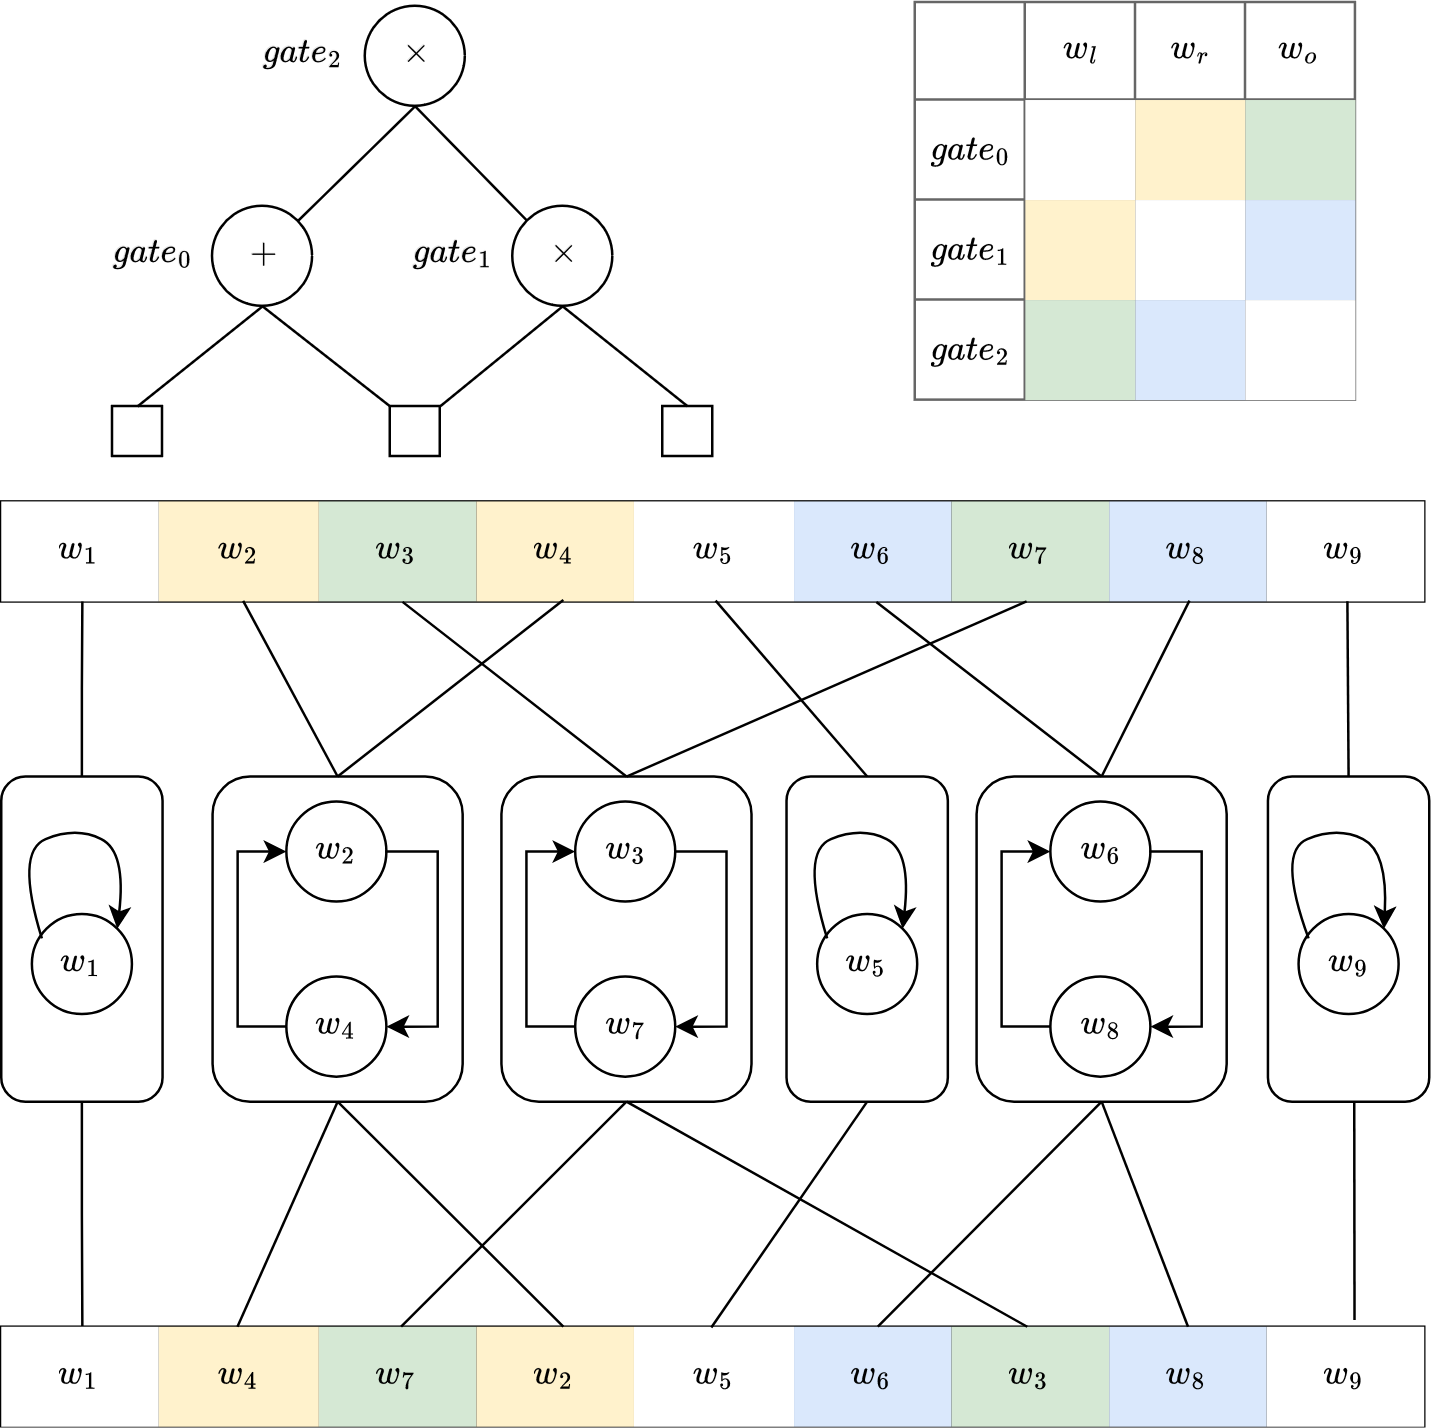
\includegraphics[width=0.75\linewidth]{round-figures/round2/permutation_function.drawio.png}
    \caption{Rotation of equivalence classes}
\end{figure}

The explicit permutation function for the example is:
$$\sigma(1) = 1, \sigma(2) = 4, \sigma(3) = 5, \sigma(4) = 2, \sigma(5) = 6, \sigma(6) = 7, \sigma(7) = 8, \sigma(8) = 3, \sigma(9) = 9$$

It might look complicated but essentially we just did a clockwise rotation on the groups of variables of the circuit. Since we have changed just the variables with equal values, the circuit should work the same as before and produce the same output. If all of the gate equations were true before the shuffling then they would succeed also after this shuffling. On the other hand, if the prover did not do the arithmetization correctly and the wiring of gates is not the same as in the former circuit this check would detect it (with very high probability). That is the core idea that will be used in the permutation check.

\hl{This should be a theorem}
Why does this correspond to the copy constraints?

In the following section we will be building the permutation check from the ground up. We will continue to work with the example circuit from \hyperref[chap:arithmetization]{arithmetization blog}. Take the vectors $w_l, w_r, w_o$ realize that permutations could be performed as intra-vector (just in a single vector) or inter-vector (between different vectors). To make out life easier we will first show how to perform a permutation check in intra-vector case and then generalize it to inter-vector check.

\begin{theorem}
\label{theorem:wire-check}
    $\forall \omega \in \Omega: p(\omega) = p(w(\omega))$ then the wire constraints are satisfied
\end{theorem}

\begin{dukaz}
    ...
\end{dukaz}

Here the only thing that remains is to show that $p(\omega) - p(w(\omega)) = 0$. However it is not that easy, since degree of the polynomial $w$ is $d$ and degree of $p$ is also $d$ their composition $p(w)$ could have degree up to $d^2$. So, if we ran this test it would force the prover to run in quadratic time with respect to $d$. Luckily there is a way to bypass this problem. Instead of this it is possible to use product check inside of set $\Omega$ using only polynomials of degree $d$ a so called plonk permutation trick. 

\begin{lemma}
    $\forall \omega \in \Omega: p(\omega) = p(w(\omega))$ if and only if $l(y,z) = 1$ where $l(y , z) = \prod_{x \in \Omega} \frac{p(x)+xw(x)+z}{p(x)+yx+z}$
\end{lemma}

\begin{dukaz}
    ...
\end{dukaz}

To prove that $l(y, z)$ indeed is equal to 1 one must show.
\begin{enumerate}
    \item verifier picks $y, z \in \mathcal{F}_p$
    \item prover build $l_1(x)$ from the mentioned lemma
    \item run product check to prove that $\prod l_1(x) = 1$
    \item validate $l_1$: run zero test on $\Omega$ to prove that $l_2(x) = 0$ zero where $l_2(x) = (p(x)+yx+z)l_1(x) - (p(x)+yw(x)+z)$
\end{enumerate}
% % \hl{need to prove correctness and all of the remaining stuff}

\subsection{Output Check}
The last one is very simple the prover just need to open the polynomial at $P(w^{3|C| -1})$ which is the output to the whole arithmetic circuit. 

\begin{lemma}{Test zero polynomial}
    For a non-zero polynomial $f \in \mathbb{F}_p^{\geq d}$ probability $Pr(f(r) = 0)$ is 
    $\frac{d}{p}$.
\end{lemma}

This observation similar to lemma 1. Depending on the choice of $d$ and $p$ the probability it negligible for practical use. This observation enable us to effectively check is commited polynomial is zero polynomial. 

% \section{Basic Interactive Protocol}
% Let's begin with a simplified description of how the proving works. In each prover round, we will create some polynomials out of the ingredients we've already computed, commit to them, and afterward evaluate (open) them at a random point. These polynomials should evaluate to 0 over the specified $H$. Checking each element of $H$ would be of course inefficient, so the problem is reduced.

% We will be using the vanishing polynomial $Z_H(x)$ which has roots as all the elements of $H$. Proving that a polynomial $p$ is zero over $H$ is the same as proving that it is divisible by $Z_H$. So, there must exists $q(x)$ such that $p(x) = q(x)Z_H(x)$. Next both $p, q$ will be committed by the KZG commitment scheme. After that, the polynomials are opened at a random point, which is given by the verifier who sampled it uniformly randomly. Finally, the verifier looks at provided commitments and openings. Thanks to the commitment scheme the verifier believes the openings of the polynomials. Then he compares the provided openings and from previous observations, we know that it is sufficient to have a single opening.


% \procedureblock{Basic Non-Interactive protocol}{%
%     \textbf{Orale} \<\< \textbf{Prover} \<\< \textbf{Verifier} \\
%     \<\< \text{get polynomials } p, q  \<\< \\
%     \< \sendmessageleft{top=polynomials,bottom=pq} \<\<\< \\
%     \< \sendmessageright{top=challenge z} \<\<\< \\
%     \<\< \text{compute evaluations}  \<\< \\
%     \<\< \text{and commitments}  \<\< \\
%     \<\<\< \sendmessageright{top=$p(z)q(z)$, bottom=$[p]_1 [q]_1$} \< \\
%     \<\<\<\< \text{verify result} \\
% }

% \begin{note}
%     To give you a simplified idea of how this works, the Fiat-Shamir heuristic transforms the interactive argument of knowledge into a digital signature. The whole idea is that the prover acts also as the verifier and tries to give queries to itself using a deterministic random function such as a cryptographic hash function. The oracle must be deterministic otherwise the verifier would not be able to reconstruct the values. The input to the random function should include all of the public information and all elements in the proof transcript up until that point inside the hash function.

%     \begin{figure}
%         \centering
%         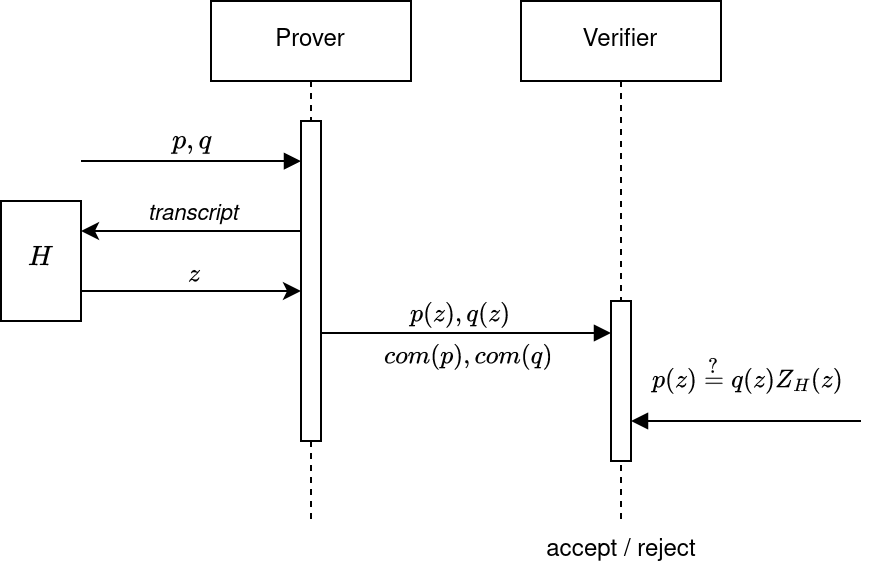
\includegraphics[width=0.75\linewidth]{round-figures/round1/proof_overview_fiat-shamir.drawio.png}
%         \caption{Sketch of Fiat-Shamir}
%     \end{figure}

%     With this knowledge, we could get back to the overview diagram and make it more detailed.
% \end{note}